\chapter{Manipulacija objektov z robotom Epson E2S651 in robotskim vidom} %
%\Large%
%\textbf{Cilj vaje} \\%
%\\%
%\normalsize%

\vspace{-3.5cm}

\begin{mdframed}[backgroundcolor=green!20, shadow=true,roundcorner=8pt]
\vspace{-0.35cm}
\section{Cilji vaje}
\begin{itemize}
\item spoznavanje uporabniškega okolja Epson RC+ za premikanje in programiranje robota Epson
\item spoznavanje ukazov za premikanje robota SCARA konfiguracije
\item sharnjevanje ciljnih točk robota
\item delo z I/O enoto
\item načina za definiranje palete
\item uporaba video sistema v kombinaciji s homogenimi transformacijami  za robotsko manipulacijo detektiranih objektov
\item spoznavanje okolja Matlab za namen preračuna homogenih transformacij
\item uporaba znanja pridobljenega na predavanjih o homogenih transformacijah med različnimi koordinatnimi sistemi
\end{itemize}
\end{mdframed}

\section{Pregled vaje}
\vspace{0.3cm}%
\underline{\textbf{1. del}} \\%

Na mizo v delovnem prostoru robota postavite zamašek in ga z robotom
oz. robotskim prijemalom primete. Prijetega odnesite nad poljubno
ustje plastenke in ga privijte.  Po krajšem premoru ga odvijte in
odnesite na začetno pozicijo. Tu ga spustite, robot pa umaknete.

\underline{\textbf{2. del}} \\%

Z uporabo robotskega vida in robota Epson E2S651 določite pozicijo
poljubno postavljenih zamaškov v delovnem prostoru robota (Slika
\ref{fScara_Del2}) in jih privijte na ustja plastenk. Pri nalogi je
potrebno izvesti postopek kalibracije s katero definirate lego
koordinatnega sistema kamere v referenčnem koordinatnem sistemu
robota. Za izračun potrebnih transformacij uporabite okolje Matlab,
za gibanje robota pa razvojno okolje Epson RC+.
%\psfull %

\begin{figure}[h]
    \centering
    \includegraphics[width=0.83\textwidth]{/Eps/000_Prvi_del.eps}
    \vspace{-0.3cm}
    \caption{Postavitev zamaškov v delovnem prostoru robota.}
    \label{fScara_Del2}
\end{figure}

\section{Lastnosti sistema}

Robot Epson E2S651 je robot tipa SCARA srednje velikosti. Njegove
najpomembnejše lastnosti kaže tabela na sliki \ref{fTabela}.

\begin{figure}[h]
    \centering
    \includegraphics[width=0.8\textwidth]{/Eps/01_Tabela.eps}
    \vspace{-0.3cm}
    \caption{Lastnosti robota Epson E2S651}
    \label{fTabela}
\end{figure}

Robot med delom v industrijskem proizvodnem procesu je prikazan na
sliki \ref{fRobot}, kjer je uporabljen kot nosilec laserskega
triangulacijskega merilnika razdalje za merjenje dimenzij ulitkov iz
sive litine. Na desni sliki \ref{fKontrolna_plosca} pa je prikazana
majhna kontrolna plošča na samem robotu, kjer najdemo priključke za
zrak in električne signale ter tudi gumb za sprostitev zavore
tretjega sklepa.


\begin{figure}[t]
    \centering
    \begin{minipage}{.4\textwidth}
        \centering
        \includegraphics[width=0.8\textwidth]{/Eps/02_Robot.eps}
        \vspace{-0.0cm}
        \caption{Robot Epson E2S651}
        \label{fRobot}
    \end{minipage}
    \begin{minipage}{.55\textwidth}
        \centering
        \includegraphics[width=0.95\textwidth]{/Eps/03_Kontrolna_plosca_na_robotu.eps}
        \caption{Kontrolna plošča na robotu}
        \label{fKontrolna_plosca}
    \end{minipage}
\end{figure}



\section{Programsko okolje Epson RC+}

\begin{figure}[b]
    \centering
    \includegraphics[width=0.82\textwidth]{/Eps/04_Programski_vmesnik_RCPlus.eps}
    \vspace{-0.3cm}
    \caption{Glavno okno programskega okolja Epson RC+}
    \label{fProgramskoOkolje}
\end{figure}

Krmilnik robota je zasnovan na industrijskem osebnem računalniku.
Osi robota vodijo neodvisni namenski procesorji, uporabniški
vmesnik Epson RC+, ki predstavlja delovno okolje za vse robote
Epson, pa teče v operacijskem sistemu Windows 2000. Vse komponente
krmilnika, vključno s končnimi stopnjami ojačevalnikov, so v
standardnem ohišju. Pisanje robotskih aplikacij poteka v
programskem jeziku SPEL (izpeljanka BASIC-a), ki nudi široke
možnosti komunikacije in vključevanja v aplikacije, razvite s
splošno namenskimi programskimi jeziki (vmesnik ActiveX, TCP/IP
itd.). Izgled vmesnika RC+ prikazuje slika
\ref{fProgramskoOkolje}.





\vspace{0.2cm}
\subsection{Osnove o pisanju programov}
\vspace{0.5cm}
\begin{enumerate}

    \item[1)] Za pisanje programa je potrebno odpreti nov projekt. To storimo tako, %
    da izberemo menu \textbf{Project} $\longrightarrow$ \textbf{New}... Pod \textbf{Select Project Folder} izberemo mapo %
    \emph{Projects$\setminus$StudentskeVaje} in v polje \textbf{New Project Name} vpišemo poljubno ime %
    projekta. \emph{Pazimo, da je vključena izbira Create Main.prg}. Izbiro potrdimo z gumbom OK.%

    \item[2)]  Odpremo pa lahko tudi že ustvarjeni projekt. To storimo tako, da izberemo menu %
    \textbf{Project} $\longrightarrow$ \textbf{Open...} Pod \textbf{Select Project to Open} %
    izberemo projekt in kliknemo gumb \textbf{OK}.%

    \item[3)]  če področje za pisanje programov še ni odprto (okno z imenom Main.prg), %
    ga odpremo tako, da v \textbf{hierarhičnem drevesu projekta dvakrat kliknemo na Main.prg}. %

    \item[4)]  Za demonstracijo pisanja programa v prazno belo polje vpišemo: \\%
        \\
\small
        \hspace*{0.0cm}   \texttt{Function Main} \\%
        \hspace*{0.3cm}   \texttt{On 0 \hspace{1.35cm} ' Zapremo prijemalo.} \\%
        \hspace*{0.3cm}   \texttt{Wait 1.0 \hspace{0.6cm} ' Počakamo 1 sekundo.} \\%
        \hspace*{0.3cm}   \texttt{Off 0 \hspace{1.15cm} ' Odpremo prijemalo.} \\%
        \hspace*{0.0cm}   \texttt{Fend} \\%
        \\
\normalsize
    S tem smo ustvarili Main funkcijo. Med Function Main in Fend pa
    vpisujemo ukaze. \emph{Za primer smo vnesli ukaz za zapiranje in
    odpiranje prijemala, vmes pa počakamo 1 sekundo.}

\begin{figure}[h]
    \centering
   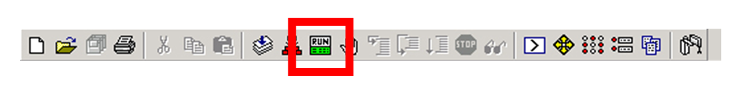
\includegraphics[width=\textwidth]{/Eps/13_Zaganjanje_programov.eps}
    \vspace{-0.9cm}
    \caption{Zaganjanje napisanih programov}
    \label{fZaganjanjePrograma}
\end{figure}

    \item[5)] Napisan program zaženemo tako, da kliknemo ikono, prikazano na sliki \\ %
    \ref{fZaganjanjePrograma}, nato pa še gumb \textbf{Start main}.%

\end{enumerate}





\subsection{Vključitev pogonskih motorjev}

Ob zagonu programskega okolja Epson RC+ pogonski motorji nimajo
napajanja. Napajanje vključimo tako, da kliknemo na ikono, ki je
označena na sliki \ref{fOrodnaVrsticaKontrolno}, nato pa se odpre
okno s slike \ref{fOrodnaVrsticaKontrolnoOkno}.

\begin{figure}[h]
    \centering
    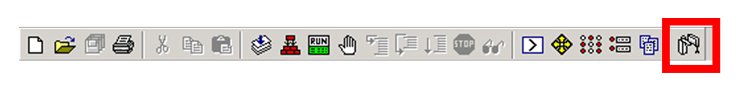
\includegraphics[width=\textwidth]{/Eps/05_Orodna_vrstica.eps}
    \vspace{-0.9cm}
    \caption{Orodna vrstica in ikona za odpiranje kontrolnega okna}
    \label{fOrodnaVrsticaKontrolno}
\end{figure}
\vspace{-0.3cm}
\begin{figure}[h]
    \centering
    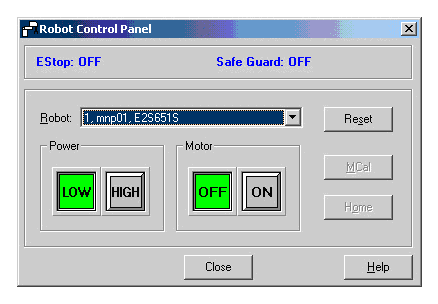
\includegraphics[width=0.9\textwidth]{/Eps/06_Kontrolno_okno.eps}
    \vspace{-0.3cm}
    \caption{Kontrolno okno robota}
    \label{fOrodnaVrsticaKontrolnoOkno}
\end{figure}


\noindent %
\textbf{\underline{Izbire oziroma gumbi  v kontrolnem oknu}} %
\\
\begin{enumerate}
    \item[-] \textbf{EStop: (OFF/ON)} \\%
        \hspace*{1.0cm}    $\longrightarrow$ Napis signalizira, ali je pritisnjena tipka \textbf{(črna škatla na mizi s \\%
        \hspace*{1.7cm}    kovinskim gumbom v sredini)} zasilnega izklopa. %
    \item[-] \textbf{Safe Guard: (OFF/ON)} \\%
        \hspace*{1.0cm}    $\longrightarrow$ Napis signalizira, ali je nekdo vstopil v varnostno kletko robota. %
    \item[-] izbira \textbf{Robot:} $\longrightarrow$ Izberemo robot (v našem primeru je samo eden). %
    \item[-] gumb \textbf{Reset} $\longrightarrow$ Resetiramo stanje po napaki ali pritisnjeni zasilni tipki. %
    \item[-] gumb \textbf{Help} $\longrightarrow$ S pritiskom prikličemo pomoč. %
    \item[-] gumb \textbf{Close} $\longrightarrow$ S pritiskom zapremo okno. %
\end{enumerate}

\noindent %
\textbf{Power}
\begin{enumerate}
    \item[-] \textbf{LOW} $\longrightarrow$ Pogonski motorji delujejo v načinu \textbf{nizke} moči. %
    \item[-] \textbf{HIGH} $\longrightarrow$ Pogonski motorji delujejo v načinu \textbf{visoke} moči. %
\end{enumerate}

\noindent %
\textbf{Motor}
\begin{enumerate}
    \item[-] \textbf{OFF} $\longrightarrow$ Izključimo napajanje pogonskih motorjev \emph{(v tem stanju lahko \\%
        \hspace*{1.5cm}    robot premikamo z roko)}. %
    \item[-] \textbf{ON} $\longrightarrow$ Vključimo napajanje pogonskih motorjev \emph{(robot lahko premikamo \\%
        \hspace*{1.3cm}    le preko uporabniškega vmesnika)}. %
\end{enumerate}



% ********************************************************************
\noindent %
\begin{mdframed}[backgroundcolor=red!80, shadow=true,roundcorner=8pt]
%\begin{tikzpicture}
%    \node [fill=red,rounded corners=5pt] {
%    \begin{minipage}{0.98\textwidth}
        \vspace{0.2cm}
        \large
\textcolor[rgb]{1.00,1.00,0.00}{\textbf{V fazi programiranja in testiranja mora biti zaradi vaše varnosti in morebitnih poškodb opreme}}\\ %
\textcolor[rgb]{1.00,1.00,0.00}{\LARGE \textbf{vedno vklopljena opcija Power LOW!}} \\ %
        \vspace{0.2cm}
\textcolor[rgb]{1.00,1.00,0.00}{\small Opcija Power High je namenjena doseganju polne dinamike robota v industrijskem okolju.} %
        \vspace{0.2cm}
%    \end{minipage}
%    };
%\end{tikzpicture}
\end{mdframed}
\normalsize
% ********************************************************************







\vspace{0.0cm}
\subsection{Upravljanje z digitalnimi vhodi in izhodi}

Krmilnik v osnovi omogoča spremljanje in upoštevanje 16 digitalnih
vhodnih signalov in 16 digitalnih izhodnih signalov. Za namen
izvajanja prijemanja pokrovčkov je na robot nameščeno pnevmatsko
prijemalo. Pnevmatski cilinder prijemala krmilimo z monostabilnim
elektropnevmatskim ventilom, ki ga krmilimo z enim digitalnim
izhodom iz robotskega krmilnika. Po pritisku na ikono s slike
\ref{fOrodnaVrsticaIO} se odpre okno s slike
\ref{fOrodnaVrsticaIOOkno}.

\begin{figure}[h]
    \centering
    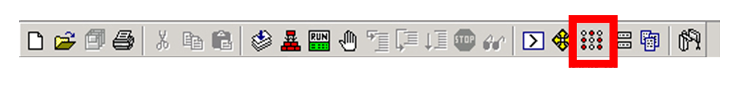
\includegraphics[width=0.99\textwidth]{/Eps/07_Orodna_vrstica_IO.eps}
    \vspace{-0.9cm}
    \caption{Orodna vrstica in ikona za odprtje okna upravljanja z digitalnimi vhodi in izhodi}
    \label{fOrodnaVrsticaIO}
\end{figure}

\begin{figure}[h]
    \centering
    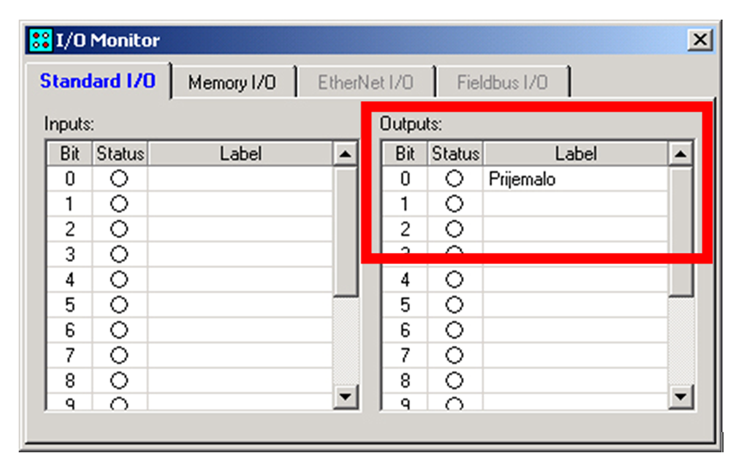
\includegraphics[width=0.85\textwidth]{/Eps/08_IO.eps}
    \vspace{-0.3cm}
    \caption{Okno za upravljanje z digitalnimi vhodi in izhodi}
    \label{fOrodnaVrsticaIOOkno}
\end{figure}


\noindent %
\textbf{\underline{Okno za upravljanje z digitalnimi vhodi in izhodi}} %
\\
\begin{enumerate}
    \item[-] \textbf{Standard I/O} $\longrightarrow$ Zavihek, kjer upravljamo z digitalnimi vhodi in izhodi. %
    \item[-] \textbf{Inputs} $\longrightarrow$ Digitalni vhodi \emph{(biti od 0 do 15)}. %
    \item[-] \textbf{Outputs} $\longrightarrow$ Digitalni izhodi \emph{(biti od 0 do 15)}. %
    \item[-] \textbf{Memory I/O} $\longrightarrow$ Zavihek za upravljanje z biti spomina (512 bitov), upo-\\%
        \hspace*{2.7cm}    rabljeni za komunikacijo med opravili (task) programa. %
\end{enumerate}


Prijemalo oziroma njegov elektropnevmatski ventil je priklopljen
na \textbf{digitalni izhod številka 0}. \textbf{Ta signal vklopimo
oziroma izklopimo z dvakratnim klikom na krogec v stolpcu Status}
(Slika \ref{fOrodnaVrsticaIOOkno}). Prijemalo je odprto, ko je
krogec prazen, in zaprto ob polnem krogcu.








\vspace{0.2cm}
\subsection{Okno za premikanje robota in učenje točk}

Robot premikamo na različne načine, spremljamo trenutno lego in
shranjujemo lego vrha robota v oknu, katerega odpremo s pritiskom na
gumb s slike \ref{fOrodnaVrsticaPremikanje}.
%okna s slike \ref{fOrodnaVrsticaPremikanjeOkno}. Okno odpremo s
\vspace{0.2cm} %
\begin{figure}[h]
    \centering
    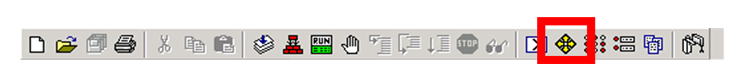
\includegraphics[width=\textwidth]{/Eps/09_Orodna_vrstica_Premikanje.eps}
    \vspace{-0.9cm}
    \caption{Orodna vrstica in ikona za okno za premikanje robota in učenje točk}
    \label{fOrodnaVrsticaPremikanje}
\end{figure}

\noindent %
\textbf{\underline{Ukazi za premikanje robota}} %
\vspace{0.5cm}
\begin{enumerate}

    \item[-] \textbf{Jog Mode} $\longrightarrow$ Izbiramo koordinatni sistem za premikanje robota (\emph{World,\\ %
        \hspace*{2.3cm}         Tool, Joint}). %
\vspace{0.2cm}
    \item[-] \textbf{Jog Distance} $\longrightarrow$ Izberemo korak premika, kjer prednastavljene korake \\%
        \hspace*{2.8cm}            izberemo s pritiskom na ustrezen krogec (Long, Medium\\%
        \hspace*{2.8cm}            ali Short). V poljih lahko vrednosti tudi spreminjamo. %
\vspace{0.2cm}
    \item[-] \textbf{Current Position} \\ %
        \hspace*{1.0cm}    $\longrightarrow$ Izpisuje se trenutna lega izbranega orodja (npr. \emph{Tool 0}) v refe-\\%
        \hspace*{1.7cm}    renčnem koordinatnem sistemu (izbira \textbf{World}). \\%
        \hspace*{1.0cm}    $\longrightarrow$ Izpisujejo se trenutni koti v sklepih v stopinjah (izbira \textbf{Joint}).\\%
        \hspace*{1.0cm}    $\longrightarrow$ Izpisujejo se trenutni pulzi enkoderjev v sklepih (izbira \textbf{Pulse}).\\%
\vspace{0.2cm}
    \item[-] \textbf{Jogging $\&$ Motion Commands} \\ %
        \hspace*{1.0cm}    $\longrightarrow$ S puščicami vodimo robot v izbrani smeri koordinatnega si-\\%
        \hspace*{1.7cm}    stema (\emph{Jog Mode = World ali Tool}) ali ga rotiramo po sklepih \\%
        \hspace*{1.7cm}  (\emph{Jog Mode = Joint}). %
\end{enumerate}

%\begin{figure}[h]
%    \centering
%    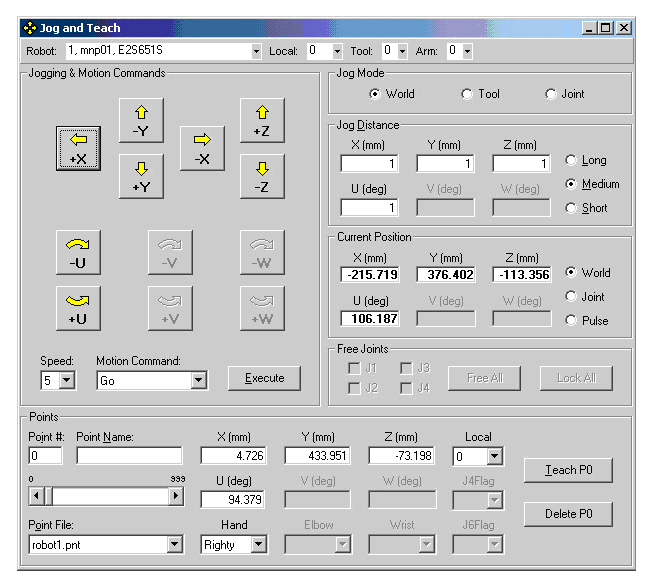
\includegraphics[width=0.97\textwidth]{Poglavja_Slike/02_SCARA_Umetni_vid/Slike/Eps/10_Premikanje.eps}
%    \vspace{-0.3cm}
%    \caption{Okno za premikanje robota in učenje točk}
%    \label{fOrodnaVrsticaPremikanjeOkno}
%\end{figure}

\begin{figure}[h]
    \centering
    \includegraphics[width=0.97\textwidth]{/Eps/11_Ukazi_za_premikanje.eps}
    \vspace{-0.3cm}
    \caption{Ukazi za premikanje robota}
    \label{fUkaziPremikanjeRobota}
\end{figure}

\noindent %
\textbf{\underline{Ukazi za učenje točk}} %

\begin{enumerate}

    \item[-] \textbf{Points} $\longrightarrow$ Razdelek omogoča shranjevanje trenutnih leg vrha robota v da- \\ %
        \hspace*{1.75cm}      toteko (\emph{Point File}); največje število točk v eni datoteki je 1000.\\ %
        \hspace*{1.75cm}      V okno Point $\#$: ročno vpišemo številko točke ali pa jo nasta- \\ %
        \hspace*{1.75cm}      vimo z drsnikom spodaj. Trenutne vrednosti lege  X, Y, Z, U \\ %
        \hspace*{1.75cm}       in Local lahko poljubno spreminjamo. \textbf{Točko shranimo} s pri- \\ %
        \hspace*{1.75cm}      tiskom na \textbf{gumb Teach P$\#$, zbrišemo} pa jo z \textbf{Delete P$\#$}. \\%

\end{enumerate}

\begin{figure}[h]
    \centering
    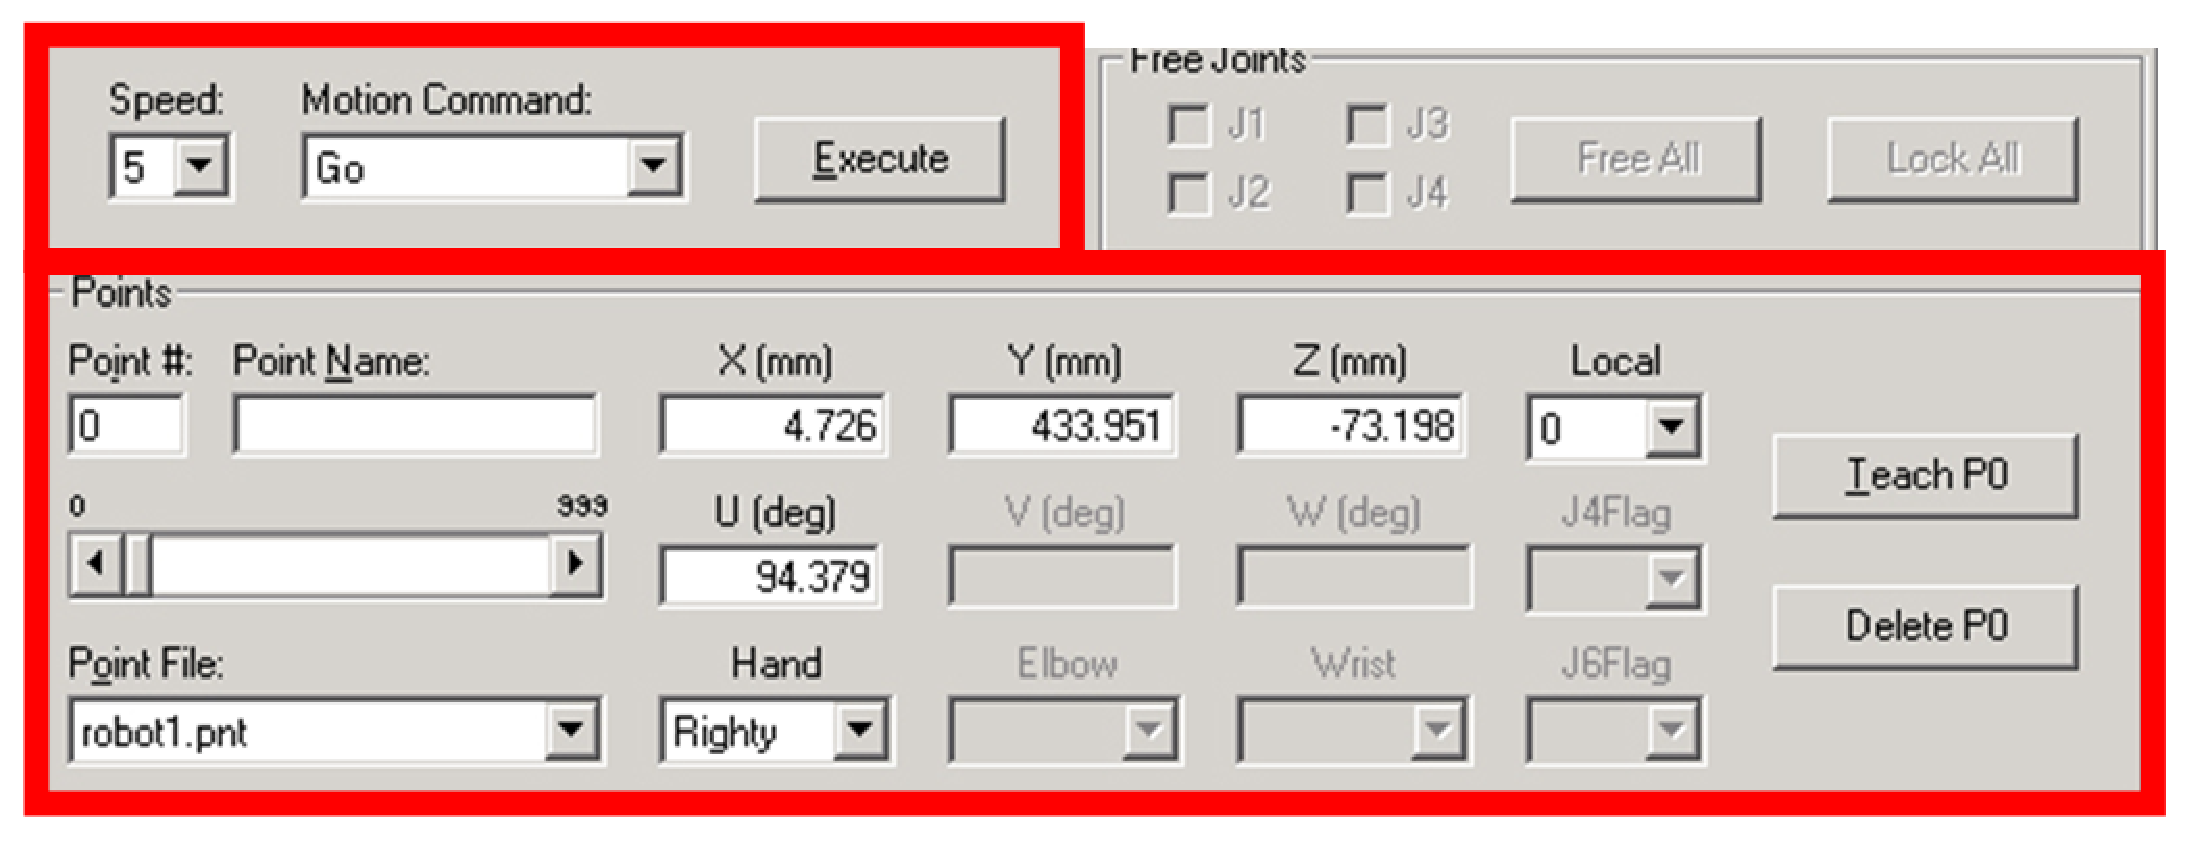
\includegraphics[width=0.9\textwidth]{/Eps/12_Ucenje_tock.eps}
    \vspace{-0.3cm}
    \caption{Ukazi za učenje točk}
    \label{fUkaziUcenjeTock}
\end{figure}


Robot lahko v shranjene lege premikamo z izbirami na sliki
\ref{fUkaziUcenjeTock}, skrajno levo zgoraj. Hitrost premika
nastavimo z izbiro \emph{Speed}, način giba z izbiro \emph{Motion
Command}, gibanje pa štartamo z gumbom \textbf{Execute}.


\vspace{0.0cm} %
\section{1. del naloge}

V 1. delu naloge spoznate ukaze in postopek za prijem zamaška,
privitje zamaška na ustje plastenke, njegovo odvitje z ustja ter
spust zamaška na začetno lego. Ta postopek je namreč večji del
programa, ki je v 2. delu naloge že napisan in ga le zaženete.

\subsection{Ukazi, potrebni za izvedbo naloge}
\vspace{0.3cm}

\begin{mdframed}[backgroundcolor=green!20, shadow=true,roundcorner=8pt]
%\begin{tikzpicture}
%    \node [fill=green,rounded corners=5pt] {
%    \begin{minipage}{0.98\textwidth}
        \vspace{0.2cm}
\textbf{Jump} $\longrightarrow$ premik vrha robota iz točke v točko (recimo iz P0 v P1), ki ga \\
\hspace*{1.6cm}  razdelimo na: \vspace*{0.3cm} \\ %
\hspace*{1.6cm} 1) translacija navzgor z nespremenjeno orientacijo; \\ %
\hspace*{1.6cm} 2) sinhrono premikanje sklepov, pri čemer se orientacija vrha \\ %
\hspace*{2.05cm} robota spremeni, če je drugačna v ciljni točki; \\ %
\hspace*{1.6cm} 3) translacija navzdol v ciljno lego z ustrezno orientacijo vrha \\%
\hspace*{2.05cm} robota. %
        \vspace{0.2cm}
%    \end{minipage}
%    };
%\end{tikzpicture}
\end{mdframed}

\begin{figure}[h]
    \center
    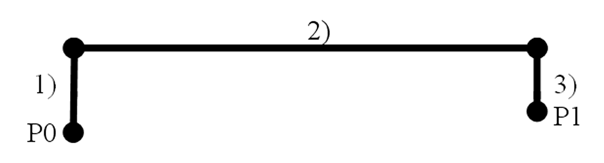
\includegraphics[width=0.65\textwidth]{/Eps/14_Jump.eps}
    \vspace{-0.3cm}
    \caption{Premikanje vrha robota pri uporabi ukaza Jump}
    \label{fJump}
\end{figure}

\begin{mdframed}[backgroundcolor=green!20, shadow=true,roundcorner=8pt]
%\begin{tikzpicture}
%    \node [fill=green,rounded corners=5pt] {
%    \begin{minipage}{0.98\textwidth}
        \vspace{0.2cm}
\textbf{Go} $\longrightarrow$ premik vrha robota iz točke v točko (P0 v P1) s sinhronim premika- \\ %
\hspace*{1.2cm} njem sklepov. Sinhrono  premikanje pomeni, da se vsi sklepi, katerih \\ %
\hspace*{1.2cm} premik je potreben, začnejo premikati hkrati in tudi hkrati končajo. \vspace*{0.3cm}\\ %
\hspace*{1.2cm} \emph{Primer: Za dosego končne lege se mora prvi segment  zarotirati za} \\ %
\hspace*{1.2cm} \emph{213$^\circ$, tretji pa translirati za 8 mm. Rotacijo prvega sklepa robot} \\ %
\hspace*{1.2cm} \emph{opravlja z nastavljeno hitrostjo v programu (največji premik), hitrost} \\ %
\hspace*{1.2cm} \emph{translacije pa prilagodi času, ki je potreben za izvršitev rotacije} \\ %
\hspace*{1.2cm} \emph{prvega sklepa.}  %
        \vspace{0.2cm}
%    \end{minipage}
%    };
%\end{tikzpicture}
\end{mdframed}

\begin{figure}[h]
    \center
    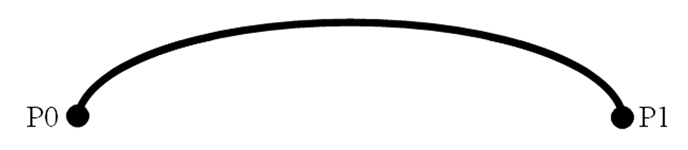
\includegraphics[width=0.65\textwidth]{/Eps/15_Go.eps}
    \vspace{-0.3cm}
    \caption{Premikanje vrha robota, ko je uporabljen ukaz Go}
    \label{fJump}
\end{figure}

\textbf{Motor P} $\longrightarrow$ Parameter (P) \textbf{On} vključi napajanje motorjev, parameter \\ %
\hspace*{2.1cm} \textbf{Off} pa napajanje izključi (\emph{primer: Motor On}). \vspace{-0.3cm} \\ %

\textbf{Power P} $\longrightarrow$ Nastavitev moči delovanja motorjev. Parameter (P) \textbf{Low} \\ %
\hspace*{2.1cm} nastavi nizek režim, parameter \textbf{High} pa večji režim moči.  \vspace{-0.3cm} \\ %

\textbf{Speed N} $\longrightarrow$ Največja hitrost (N) gibanja v odstotkih (od 1 $\%$ do 100 $\%$) glede \\ %
\hspace*{2.1cm}   na maksimum (\emph{primer: Speed 40}). \vspace{-0.3cm} \\ %

\textbf{Accel N,M} $\longrightarrow$ Največji pospešek (N) in pojemek (M) v odstotkih (od 1 $\%$ do\\ %
\hspace*{2.4cm} 100 $\%$) glede na maksimum (\emph{primer: Accel 30, 10}). \vspace{-0.3cm} \\ %

\textbf{On N} $\longrightarrow$ Dvig digitalnega signala na naslovu N (\emph{primer: On 0}). \vspace{-0.3cm} \\ %

\textbf{Off N} $\longrightarrow$ Spust digitalnega signala na naslovu N (\emph{primer Off 0}). \vspace{-0.3cm} \\ %

\textbf{Wait N} $\longrightarrow$ Ustavitev izvajanja programa za N sekund (\emph{primer: Wait 1.3}). \vspace{-0.3cm} \\ %


\subsection{Koraki za izvedbo naloge}
\vspace{0.3cm}

\begin{mdframed}[backgroundcolor=green!20, shadow=true,roundcorner=8pt]
%\begin{tikzpicture}
%    \node [fill=green,rounded corners=5pt] {
%    \begin{minipage}{0.98\textwidth}
        \vspace{0.2cm}
\noindent %
\textbf{Napišite program (primer spodaj) za premik robota iz točke P0 v P1, prijem zamaška in njegov prenos nad ustje plastenke v točki P2. Sledi privijanje v točko P3. Po krajši pavzi vrstni red nalog obrnite in odložite zamašek na izhodiščno pozicijo, robot pa naj se vrne v izhodiščno točko P0. Vsaka operacija prijemanja in spuščanja zamaška zahteva kratke premore, zato uporabite ukaz Wait.} \\ %
\\
\\
\small
\texttt{Function main} \\%
    \hspace*{0.3cm}   \texttt{Motor On        \small\hspace{0.75cm} ' Vključitev napajanja motorjev.} \\%
    \hspace*{0.3cm}   \texttt{Power Low       \small\hspace{0.55cm} ' Nizka moč delovanja motorjev.} \\%
    \hspace*{0.3cm}   \texttt{Speed 20        \small\hspace{0.75cm} ' Hitrost gibanja na 20$\%$ največje.} \\%
    \hspace*{0.3cm}   \texttt{Accel 20, 20    \small\hspace{0.00cm} ' Pospešek in pojemek na 20$\%$ največjega.} \\%
    \hspace*{0.3cm}   \texttt{Off 0           \small\hspace{1.35cm} ' Preventivno odprtje prijemala.} \\%
    \hspace*{0.3cm}   \texttt{Wait 0.2        \small\hspace{0.80cm} ' Pavza 0.2 sekunde.} \\%
     \\%
    \hspace*{0.3cm}   \texttt{Go P0           \small\hspace{1.40cm} ' Premik robota v točko P0.} \\%
    \hspace*{0.3cm}   \texttt{Jump P1         \small\hspace{1.00cm} ' Premik robota v točko P1.} \\%
    \hspace*{0.3cm}   . \\%
    \hspace*{0.3cm}   . \\%
    \hspace*{0.3cm}   . \\%
\texttt{Fend} \\%
\normalsize

%    \end{minipage}
%    };
%\end{tikzpicture}
\end{mdframed}

\begin{mdframed}[backgroundcolor=blue!20, shadow=true,roundcorner=8pt]
%\begin{tikzpicture}
%    \node [fill=blue,rounded corners=5pt] {
%    \begin{minipage}{0.98\textwidth}
        \vspace{0.2cm}
\hspace*{0.05cm} 1) Ustvarite nov projekt (Projects$\setminus$StudentskeVaje) in vpišite njegovo ime v \\ %
\hspace*{0.50cm} polje, ki ga razvojno okolje ponudi. \vspace*{0.3cm} \\ %
\hspace*{0.05cm} 2) V oknu za programiranje zapišete \texttt{Function main} in dve vrstici \\ %
\hspace*{0.5cm} nižje še \texttt{Fend}.  \vspace*{0.3cm} \\ %
\hspace*{0.05cm} 3) Robot ne sme imeti vključenega napajanja motorjev (Slika \ref{fOrodnaVrsticaKontrolnoOkno}). \vspace*{0.3cm} \\ %
\hspace*{0.05cm} 4) Odprite okno Jog and Teach s klikom na ustrezno ikono (Slika \ref{fOrodnaVrsticaPremikanje}). \vspace*{0.3cm} \\ %
\hspace*{0.05cm} 5) Odprite okno I/O Monitor (Slika \ref{fOrodnaVrsticaIOOkno}) in preverite, če je prijemalo odprto \\ %
\hspace*{0.5cm} (izhodni naslov 0 ne sme biti izbran). \vspace*{0.3cm} \\ %
\hspace*{0.05cm} 6) Na mizo v delovnem prostoru robota postavite zamašek. \vspace*{0.3cm} \\ %
\hspace*{0.05cm} 7) Robot ročno postavite v poljubno lego v delovnem prostoru robota. \vspace*{0.3cm} \\ %
\hspace*{0.05cm} 8) V oknu Jog and Teach (Slika \ref{fUkaziUcenjeTock}) shranite lego robota kot točko P0. \vspace*{0.3cm} \\ %
\hspace*{0.05cm} 9) Robot z roko postavite tako, da lahko prime zamašek (lega, ki ji sledi \\ %
\hspace*{0.5cm} stisk prijemala). Za vertikalni premik tretjega segmenta sprostite zavoro \\ %
\hspace*{0.5cm} s pritiskom na bel gumb (Slika \ref{fKontrolna_plosca}). \vspace*{0.3cm} \\ %
10) V oknu Jog and Teach (Slika \ref{fUkaziUcenjeTock}) shranite lego robota kot točko P1. \vspace*{0.3cm} \\ %
11) V oknu I/O Monitor (Slika \ref{fOrodnaVrsticaIOOkno}) kliknite na naslov izhodnega digitalnega \\ %
\hspace*{0.55cm} signala 0 za stisk prijemala. \vspace*{0.3cm} \\ %
12) Robot s prijetim zamaškom z roko premaknite tik nad ustje plastenke. \\ %
\hspace*{0.55cm} Za vertikalni premik tretjega segmenta sprostite zavoro s pritiskom na \\ %
\hspace*{0.55cm} bel gumb (Slika \ref{fKontrolna_plosca}). \vspace*{0.3cm} \\ %
13) V oknu Jog and Teach (Slika \ref{fUkaziUcenjeTock}) shranite lego robota kot točko P2.  \vspace*{0.3cm} \\ %
14) Zadnjo os robota s prijetim zamaškom z roko rotirajte (vrtite) in \\ %
\hspace*{0.55cm} vertikalno translirajte (pomik navzdol), da privijete zamašek.  Za \\ %
\hspace*{0.55cm} vertikalni premik tretjega segmenta sprostite zavoro s pritiskom na \\ %
\hspace*{0.55cm} bel gumb (Slika \ref{fKontrolna_plosca}). \vspace*{0.3cm} \\ %
15) V oknu Jog and Teach (Slika \ref{fUkaziUcenjeTock}) shranite lego robota kot točko P3. \vspace*{0.3cm} \\ %
16) V oknu I/O Monitor (Slika \ref{fOrodnaVrsticaIOOkno}) kliknite na naslov izhodnega digitalnega \\ %
\hspace*{0.55cm} signala 0 za spust zamaška. \vspace*{0.3cm} \\ %
17) Robot z roko umaknite iznad ustja plastenke. %
%    \end{minipage}
%    };
%\end{tikzpicture}
\end{mdframed}



\newpage
\section{Matlab in umetni vid}
\vspace{0.3cm}

Programsko okolje Matlab s svojo široko paleto funkcij in orodij
omogoča tudi učinkovito delo z umetnim vidom oziroma obdelavo slik
ter vzorcev. Pri vaji sta pomembni predvsem naslednji orodji:
\vspace*{0.2cm} %
\begin{enumerate}
\item[1)] \textbf{Image Acquisition Toolbox} $\longrightarrow$ skrbi za zajem slike in videa ter strojno \\%
\hspace*{5.1cm} podporo. \\ %
\vspace*{-0.37cm} %
\item[2)] \textbf{Image Processing Toolbox}  $\longrightarrow$ obdelava slike, razpoznavanje vzorcev,\\%
\hspace*{5.0cm} transformacije, ugotavljanje najrazlič-\\%
\hspace*{5.0cm} nejših lastnosti slik itd. \\ %
\end{enumerate}

Matlab je v osnovi namenjen za numerično računanje, še posebej
manipulaciji matričnih funkcij. Sliko lahko predstavimo kot
matriko. Sivinska je zapisana kot M$\times$N matrika (Slika
\ref{fMatrikaA}), barvna pa kot kot M$\times$N$\times$3 matrika,
kjer tretja dimenzija predstavlja posamezno RGB komponento (Slika
\ref{fMatrikaB}).

\begin{figure}[h]
  \begin{center}
    \subfigure[Matrika sivinske slike dimenzije M$\times$N]
    {
        \label{fMatrikaA}
        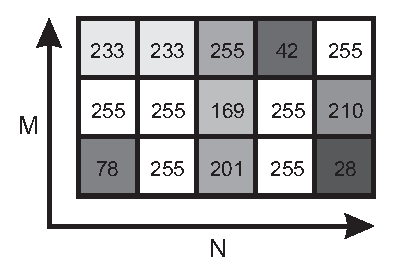
\includegraphics[scale=0.8]{/Eps/16_Sivinjska_slika.eps}
    }
    \subfigure[Matrika barvne slike dimenzije M$\times$N$\times$3]
    {
        \label{fMatrikaB}
        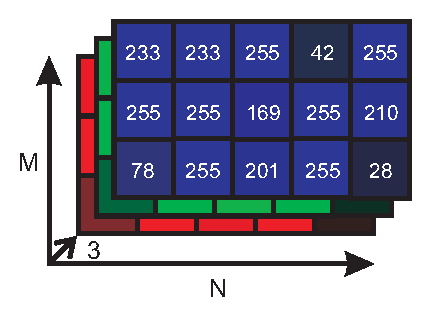
\includegraphics[scale=0.8]{/Eps/17_Barvna_slika.eps}
    } \\
  \end{center}
  \vspace{-0.5cm}
  \caption{Primera matrik sivinske in barvne slike}
  \label{fMatrike}
\end{figure}


\vspace{0.0cm}
\subsection{Video sistem}
\vspace{0.3cm}


\begin{figure}[h]
    \center
    \includegraphics[width=0.7\textwidth]{/Eps/18_Kamera.eps}
    \vspace{-0.3cm}
    \caption{Video sistem nad mizo robota}
    \label{fKamera}
\end{figure}

\noindent%
Karakteristike video sistema s slike \ref{fKamera} so:

\begin{itemize}
    \item \vspace*{-0.1cm} kamera The Imaging source DMK 21AF04 s Firewire vodilom, %
    \item \vspace*{-0.1cm} slikovni senzor CCD velikosti 640$\times$480 slikovnih elementov, %
    \item \vspace*{-0.1cm} 256 sivinskih odtenkov, %
    \item \vspace*{-0.1cm} digitalen zajem in prenos slike, %
    \item \vspace*{-0.1cm} objektiv z 8 mm goriščne razdalje. %
\end{itemize}



\subsection{2. del naloge }

\begin{mdframed}[backgroundcolor=green!20, shadow=true,roundcorner=8pt]
%\begin{tikzpicture}
%    \node [fill=green,rounded corners=5pt] {
%    \begin{minipage}{0.98\textwidth}
        \vspace{0.2cm}
Na sliki \ref{fPostavitevKS} so predstavljeni vsi nastopajoči
koordinatni sistemi. Najosnovnejši je \textbf{referenčni koordinatni
sistem robota}, ki leži v prvem sklepu robota Epson. V verigi robota
nastopa še \textbf{koordinatni sistem vrha robota}, ki je pripet na
zadnji sklep robota. Ker v sistem hočemo vključiti še informacije
dobljene s slike video kamere, v ogljišče njenega vidnega polja
pripnemo \textbf{koordinatni sistem kamere}. V vidnem polju kamere
bodo postavljeni objekti, ki imajo svojo lego (pozicijo in
orientacijo). Zato zaradi splošnosti tudi objektu v vidnem polju
kamere pripnemo \textbf{ koordinatni sistem objekta}.
%    \end{minipage}
%    };
%\end{tikzpicture}
\end{mdframed}

\begin{figure}[h]
    \center
    \includegraphics[width=0.65\textwidth]{/Eps/19_Koordinatni_sistemi.eps}
    \vspace{-0.3cm}
    \caption{Postavitev koordinatnih sistemov}
    \label{fPostavitevKS}
\end{figure}



\begin{figure}[t]
    \center
    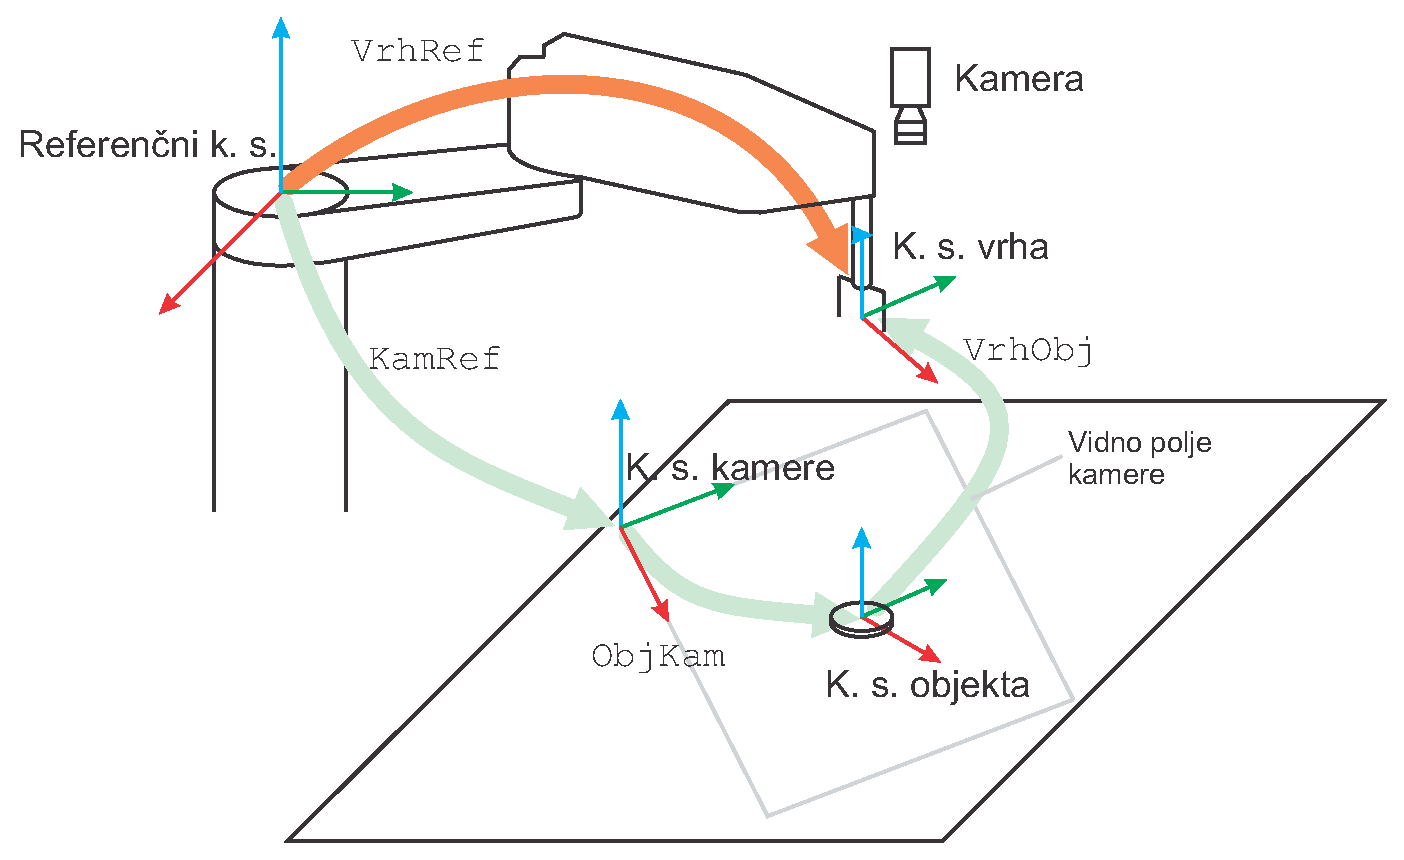
\includegraphics[width=0.8\textwidth]{/Eps/20_Transformacije_slo.eps}
    \vspace{-0.3cm}
    \caption{Transformacije med koordinatnimi sistemi}
    \label{fTransformacija}
\end{figure}

\vspace*{-0.5cm} %

\begin{mdframed}[backgroundcolor=green!20, shadow=true,roundcorner=8pt]
%\begin{tikzpicture}
%    \node [fill=green,rounded corners=5pt] {
%    \begin{minipage}{0.98\textwidth}
        \vspace{0.2cm}
Na sliki \ref{fTransformacija} so prikazane transformacije med
omenjenimi koordinatnimi sistemi. Najbolj očitna je transformacija,
ki ponazarja \textbf{lego koordinatnega sistema vrha v referenčnem
koordinatnem sistemu robota} in je odvisna od spremenljivk (koti in
pozicije) v sklepih robota.
\\
\\
Lego vrha robota lahko izrazimo oz. izračunamo tudi drugače, vendar
je potrebno poznati naslednje homogene transformacijske matrike:
\vspace*{-0.2cm} %
\begin{itemize}
    \item[-] lego koordinatnega sistema kamere v referenčnem koordinatnem sistemu robota (KamRef),\vspace*{-0.7cm} \\ %
    \item[-] lego koordinatnega sistema objekta v koordinatnem sistemu video kamere (ObjKam)\vspace*{-0.7cm}\\ %
    \item[-] lego vrha robota v koordinatnem sistemu objekta (VrhObj).\\%
\end{itemize}
\vspace*{-0.2cm} %
Omenjeno enakost zapišemo v obliki matrične
enačbe:

\begin{center}
\textbf{VrhRef = KamRef $\bullet$ ObjKam $\bullet$ VrhObj}\\ %
\end{center}
\vspace*{-0.3cm}
%\end{minipage}
%    };
%\end{tikzpicture}

\end{mdframed}

\vspace*{0.3cm}%
Razlaga okrajšav uporabljenih koordinatnih sistemov:
\vspace*{-0.2cm}%
\begin{itemize}
    \item[] \vspace*{-0.1cm} \textbf{VrhRef} $\longrightarrow$ Lega vrha robota v referenčnem koordinatnem sistemu.\\%
    \hspace*{2.0cm} \emph{Lego odčitamo v okolju Epson RC+ (okno na sliki \ref{fUkaziUcenjeTock})}. %
    \item[] \vspace*{-0.2cm} \textbf{KamRef} $\longrightarrow$ Lega koordinatnega sistema kamere v referenčnem \\ %
    \hspace*{2.15cm} koordinatnem sistemu robota.\\
    \item[] \vspace*{-0.7cm} \textbf{ObjKam} $\longrightarrow$ Lega koordinatnega sistema objekta v koordinatnem \\ %
    \hspace*{2.2cm} sistemu robota.\\
    \item[] \vspace*{-0.7cm} \textbf{VrhObj} $\longrightarrow$ Lega koordinatnega sistema vrha robota (prijemala) v \\ %
    \hspace*{2.2cm} koordinatnem sistemu objekta.\\
\end{itemize}



\begin{figure}[t]
    \center
    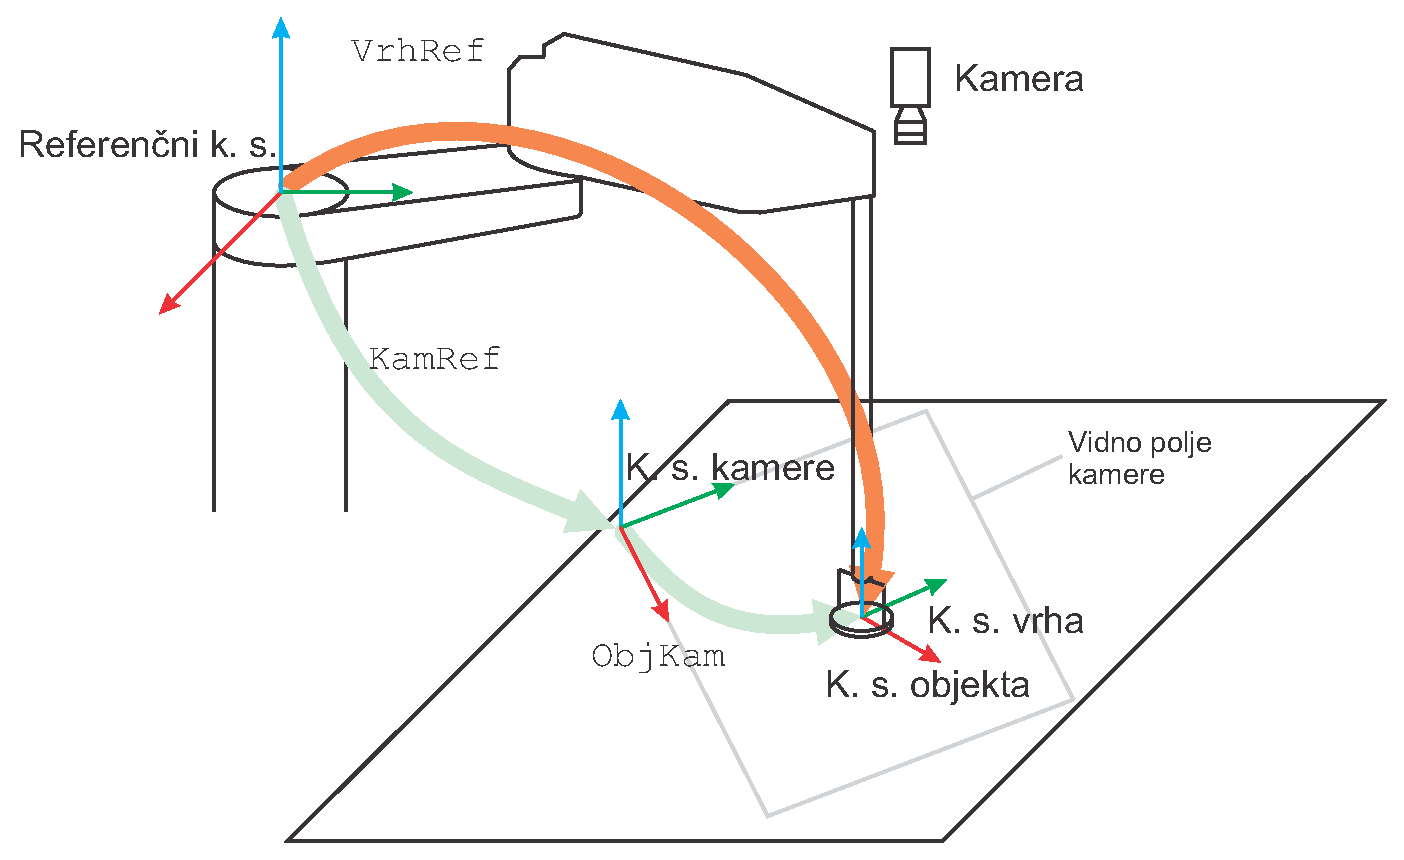
\includegraphics[width=0.8\textwidth]{/Eps/20_Transformacije_prijem_slo.eps}
    \vspace{-0.3cm}
    \caption{Transformacije med koordinatnimi sistemi pri prijemu objekta}
    \label{fTransformacijaPrijem}
\end{figure}

\noindent %
\begin{mdframed}[backgroundcolor=green!20, shadow=true,roundcorner=8pt]
%\begin{tikzpicture}
%    \node [fill=green,rounded corners=5pt] {
%    \begin{minipage}{0.98\textwidth}
        \vspace{0.2cm}
Ko robot prime objekt, želimo poravnavo koordinatnega sistema vrha
in koordinatnega sistema objekta. V tem primeru transformacija
VrhObj izgine oz. matematično gledano matrika postane enotska
matrika (po diagonali 1).
\\
\\
V tem primeru se enačba s prejšnje strani malenkostno poenostavi:

\begin{equation}
\centering
\textbf{VrhRef = KamRef $\bullet$ ObjKam $\bullet$ I} %
\label{eEqSimple}
\end{equation}

Enačba \ref{eEqSimple} opisuje lego koordinatnega sistema vrha
robota v referenčnem koordinatnem sistemu (VrhRef) ob prijemu
objekta. Uporabna je v primeru, če poznamo lego koordinatnega
sistema objekta v koordinatnem sistemu kamere (ObjKam) in lego
koordinatnega sistema kamere v referenčnem koordinatnem sistemu
robota (KamRef). Tako lahko izračunamo lego koordinatnega sistema
objekta v referenčnem koordinatnem sistemu robota in v to lego lahko
pošljemo vrh robota (VrhRef).
\\
\\
\textbf{če hočemo robot premakniti v neko lego (VrhRef) v vidnem
polju kamere in tako prijeti objekt (VrhObj = I), je potrebno
poznati obe transformaciji na desni strani enačbe (KamRef in
ObjKam). Vendar pa ob pričetku izvajanja naloge ni poznana ne ena ne
druga lega.}
\\
\\
V nadaljevanju bomo pokazali, da je določitev \textbf{ObjKam }iz
slike preprosto opravilo. Enako velja za določitev \textbf{VrhRef}.
Na podlagi teh dveh določitev lahko iz enačbe \ref{eEqSimple}
izrazimo kot neznanko \textbf{KamRef} in jo tako izračunamo. Šele
nato lahko zgornjo enačbo uporabljamo za izračun \textbf{VrhRef}, ki
premakne robot v lego za prijem objekta, katerega lego smo določili
iz slike kamere.
%\end{minipage}
%    };
%\end{tikzpicture}
\end{mdframed}

\noindent %
\textbf{\underline{Določitev matrike ObjKam}} %
%\textbf{\underline{Določitev T_obj2cam}} %
\\
~\\
Za določitev lege koordinatnega sistema objekta v koordinatnem
sistemu kamere (\textbf{ObjKam}) uporabimo plastično ploščo s tremi
črnimi pikami (Slika \ref{fKalibracijskiList}). Ena pika predstavlja
koordinatno izhodišče O, ostali dve pa ležita na \emph{x} in
\emph{y} osi koordinatnega sistema objekta.

\vspace{0.1cm}
\begin{mdframed}[backgroundcolor=red!80, shadow=true,roundcorner=8pt]
%\begin{tikzpicture}
%    \node [fill=red,rounded corners=5pt] {
%    \begin{minipage}{0.93\textwidth}
        \vspace{0.1cm}
        \center
        \large
\textcolor[rgb]{1.00,1.00,0.00}{\LARGE\textbf{POKLIčI ASISTENTA!}}\\ %
\textcolor[rgb]{1.00,1.00,0.00}{\large Asistent naj na mizico pritrdi plastično ploščo za kalibracijo.} \\ %
%    \end{minipage}
%    };
%\end{tikzpicture}
\end{mdframed}
\vspace{0.1cm}

\begin{figure}[h]
    \center
    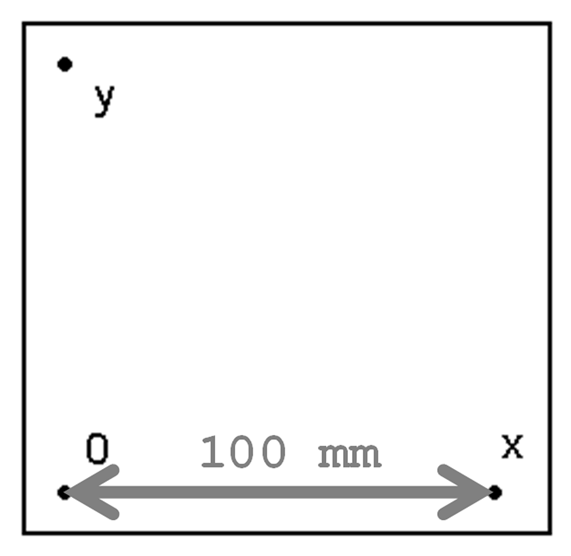
\includegraphics[width=0.6\textwidth]{/Eps/21_Kalibracijski_list}
    \vspace{-0.3cm}
    \caption{Kalibracijska plošča s točkami, ki predstavljajo k.s. objekta.}
    \label{fKalibracijskiList}
\end{figure}


\noindent %
\begin{mdframed}[backgroundcolor=blue!20, shadow=true,roundcorner=8pt]
%\begin{tikzpicture}
%    \node [fill=blue,rounded corners=5pt] {
%    \begin{minipage}{0.98\textwidth}
        \vspace{0.2cm}
        \textbf{List predstavlja objekt s koordinatnim sistemom in izhodiščem  v točki
        \emph{O}.}\\\\
        \textbf{Razdalja med točkami \emph{O} in \emph{X} ter \emph{O} in
        \emph{Y} znaša 100 mm in jo uporabimo za pretvorbo števila slikovnih elementov v milimetre.}
        \vspace{0.2cm}
%    \end{minipage}
%    };
%\end{tikzpicture}

\end{mdframed}
\normalsize

\noindent %
\textbf{Postopek za določitev matrike ObjKam} %
\\
Postopek za določanje matrike \textbf{ObjKam} je opisan v spodnjih
točkah. Pri delu uporabite programsko okolje Matlab.

\begin{enumerate}
\item[1)]  V okolju Matlab je potrebno izbrati delovno mapo
\textbf{C:$\setminus$Epson SCARA$\setminus$OR$\setminus$Epson$\_$kamera$\setminus$} in v  %
ukazni vrstici naložiti kalibracijo kamere. To storite z ukazom: \\ %
\vspace{-0.1cm}\\%
%\textbf{$\gg$ load($\bm{'}$cameraParams.mat$\bm{'}$)} \verb"Enter" \\ %\Enter
\textbf{$\gg$ load($\bm{'}$cameraParams.mat$\bm{'}$)} \verb"Enter" \\ %\Enter
\vspace{-0.2cm}\\%
%Toolbox je namenjen ugotavljanju parametrov kamere oz. uporabljenega
%objektiva (uporaba kalibracijskih vzorcev). Po potrditvi ukaza
%\emph{calib$\_$gui} se odpre okno, kjer kliknete gumb \emph{Standard
%(all the images are stored in memory)}. Postopek je že opravljen,
%zato kliknete gumb \emph{Load} in s tem naložite rezultate zadnje
%kalibracije. Trenutno prikazano okno zaprete s klikom na gumb
%\emph{Exit}.
V datoteki \textit{cameraParams.mat} so shranjene informacije o kameri in uporabljenem objektivu.
\vspace*{0.4cm} %

\item[2)] V naslednjem koraku je potrebno zajeti sliko s kamere in z ravnokar naloženimi %
parametri odstraniti popačenje objektiva. To storite tako, da v ukazno vrstico okolja %
Matlab vpišete: \\ %
\vspace{-0.3cm}\\%
\textbf{$\gg$ snapcalib2} \verb"Enter" \\ %\Enter
\vspace{-0.1cm}\\%
če je kamera pravilno priključena, se na zaslonu izpišejo parametri
kamere, kmalu zatem pa se pojavi okno z živo sliko.
\textbf{Postavite kalibracijsko ploščo v vidno polje kamere, da so na
sliki vidne vse tri točke. Sliko zajamete s pritiskom na tipko}
\verb"Enter". Slika se shrani kot calib$\_$image.tif, opravi se %\Enter
transformacija odstranjevanja popačenje objektiva in popravljena
slika se shrani kot calib$\_$image$\_$rect.tif.
\vspace*{0.2cm} %

\item[3)] Na zajeti in upragovljeni bitni sliki je potrebno ročno pokazati, kje se  %
pike koordinatnega sistema objekta (\emph{O}, \emph{X}, \emph{Y})  nahajajo. V ukazni vrstici okolja %
Matlab izvršite ukaz: \\ %
\vspace{-0.3cm}\\%
\textbf{$\gg$ select$\_$dots} \verb"Enter" \\ %%\Enter
\vspace{-0.1cm}\\%
Na prikazani bitni sliki pokažete pike z dvojnim klikom v okroglo
področje posamezne pike. \textbf{Vrstni red dvojnih klikom mora biti sledeč:
najprej dvojni klik na  točko \emph{O}, zatem dvojni klik na točko \emph{X} in še dvojni klik na točko \emph{Y}}. Pri izbiranju točk ni potrebna velika točnost, %
pomembno je le, da kliknete v območje pike, saj program sam izračuna središče. Po izbranih %
vseh treh točkah program središča točk obarva z rdečo piko. če središča odstopajo preveč %
izven belega področja pik, postopek iz te točke ponovite. \\%
\\
\noindent %
\begin{mdframed}[backgroundcolor=blue!20, shadow=true,roundcorner=8pt]
%\begin{tikzpicture}
%    \node [fill=blue,rounded corners=5pt] {
%    \begin{minipage}{0.93\textwidth}
        \vspace{0.1cm}
        Koordinate točk v koordinatnem sistemu kamere se shranijo v vektor \textbf{g} (Enačba \ref{eVektorG}). %
        \textbf{Vrednosti v vektorju g so v enotah %
        \emph{slikovni elementi}, zato jih je potrebno naknadno pretvoriti v milimetre.} %
        \vspace{0.1cm}
%    \end{minipage}
%    };
%\end{tikzpicture}
\end{mdframed}

\normalsize %
        \begin{equation}
            \textbf{g} =
            \begin{bmatrix}
                (O_x, O_y)  \\%
                (X_x, X_y)  \\%
                (Y_x, Y_y)  \\%
            \end{bmatrix}
            \label{eVektorG}
        \end{equation}
\vspace*{0.2cm} %


\item[4)] V Matlab-u odprete datoteko
(File$\longrightarrow$Open...) \textbf{zamaski2.m} in jo dopolnite:
\\ %
\\ %
\small %
\textcolor[rgb]{0.50,0.50,0.50}{\texttt{$\%$ Razdalja v slikovnih elementih med zajeto O in X točko.}} \\%
\texttt{Ox = \emph{...};} \hspace{1cm} \textcolor[rgb]{0.50,0.50,0.50}{\texttt{$\%$ Izluščimo koordinato x točke O.}} \\%
\texttt{Oy = \emph{...};} \hspace{1cm} \textcolor[rgb]{0.50,0.50,0.50}{\texttt{$\%$ Izluščimo koordinato y točke O.}} \\%
\texttt{Xx = \emph{...};} \hspace{1cm} \textcolor[rgb]{0.50,0.50,0.50}{\texttt{$\%$ Izluščimo koordinato x točke X.}} \\%
\texttt{Xy = \emph{...};} \hspace{1cm} \textcolor[rgb]{0.50,0.50,0.50}{\texttt{$\%$ Izluščimo koordinato y točke X.}} \\%
\\
\textcolor[rgb]{0.50,0.50,0.50}{\texttt{$\%$ Izračun števila slikovnih elementov med točkama O in X.}} \\%
%\texttt{d = sqrt( ( Xx - Ox  )$^\wedge$2 + (Xy - Oy )$^\wedge$2);}\\%
\texttt{d = \emph{... TUKAJ ZAPIŠETE PRAVILNO KODO;}}\\%
\\
\textcolor[rgb]{0.50,0.50,0.50}{\texttt{$\%$ Izračunamo faktor pretvorbe št. slikovnih elementov v }} \\%
\textcolor[rgb]{0.50,0.50,0.50}{\texttt{$\%$ 1 mm. Razdaljo 100 mm med pikami delimo s številom}} \\%
\textcolor[rgb]{0.50,0.50,0.50}{\texttt{$\%$ slikovnih elementov med točkami.}} \\%
\texttt{faktor = \emph{... TUKAJ ZAPIŠETE PRAVILNO KODO;};} \\ %
\\
\textcolor[rgb]{0.50,0.50,0.50}{\texttt{$\%$ Koordinate točk O,X,Y iz slikovnih elementov pretvorimo v}} \\%
\textcolor[rgb]{0.50,0.50,0.50}{\texttt{$\%$ metrične enote (v našem primeru v milimetre).}} \\%
\texttt{g$\_$mm = \emph{... TUKAJ ZAPIŠETE PRAVILNO KODO;};} \\ %
\texttt{Ox$\_$mm = \emph{...};} \hspace{0.6cm} \textcolor[rgb]{0.50,0.50,0.50}{\texttt{$\%$ Izluščimo koordinato x točke O v mm.}} \\%
\texttt{Oy$\_$mm = \emph{...};} \hspace{0.6cm} \textcolor[rgb]{0.50,0.50,0.50}{\texttt{$\%$ Izluščimo koordinato y točke O v mm.}} \\%
\texttt{Xx$\_$mm = \emph{...};} \hspace{0.6cm} \textcolor[rgb]{0.50,0.50,0.50}{\texttt{$\%$ Izluščimo koordinato x točke X v mm.}} \\%
\texttt{Xy$\_$mm = \emph{...};} \hspace{0.6cm} \textcolor[rgb]{0.50,0.50,0.50}{\texttt{$\%$ Izluščimo koordinato y točke X v mm.}} \\%
\\
\textcolor[rgb]{0.50,0.50,0.50}{\texttt{$\%$ Izračunamo kot zasuka koordinatnega sistema Objekta}} \\%
\textcolor[rgb]{0.50,0.50,0.50}{\texttt{$\%$ glede na k.s. Kamere (\ref{fTransfOK}).}} \\%
%\texttt{fiOK = atan2( (Xy$\_$mm - Oy$\_$mm ) , (Xx$\_$mm - Ox$\_$mm ) );} \\ %
\texttt{fiOK = \emph{... TUKAJ ZAPIŠETE PRAVILNO KODO};} \\ %
\\
\textcolor[rgb]{0.50,0.50,0.50}{\texttt{$\%$ Zapišemo transformacijsko matriko ObjKam - translacija}} \\%
\textcolor[rgb]{0.50,0.50,0.50}{\texttt{$\%$ D(Ox$\_$mm, Oy$\_$mm) in rotacija okrog osi Z za kot fiOK.}} \\%
\texttt{ObjKam = \emph{... TUKAJ ZAPIŠETE PRAVILNO KODO};} \\ %
%\texttt{ObjKam = [cos(fiOK), -sin(fiOK), 0, Ox$\_$mm; sin(fiOK), \\\hspace*{1.9cm}cos(fiOK), 0, Oy$\_$mm; 0, 0, 1, 0; 0, 0, 0, 1 ];} \\ %
\end{enumerate}
\normalsize %
Zgornji zapis v matrični obliki izgleda tako:
\\
\begin{equation}
    \textbf{ObjKam} =
    \begin{bmatrix}
        \textbf{cos(fiOK)}  &   \textbf{-sin(fiOK)}   &    \textbf{0}  &   \emph{Ox$\_$mm}    \\%
        \textbf{sin(fiOK)}  &   \hspace{0.1cm} \textbf{cos(fiOK)}   &    \textbf{0}  &   \emph{Oy$\_$mm}    \\%
        \textbf{0}              &   \textbf{0}                &    \textbf{1}  &   \emph{0}    \\%
        0              &   0                &    0  &   1     \\%
    \end{bmatrix}
    \label{eObjKam}
\end{equation}
\\
\begin{mdframed}[backgroundcolor=blue!20, shadow=true,roundcorner=8pt]
%\begin{tikzpicture}
%    \node [fill=blue,rounded corners=5pt] {
%    \begin{minipage}{0.93\textwidth}
        \vspace{0.1cm}
Enačba \ref{eObjKam} predstavlja transformacijsko matriko
\textbf{ObjKam} in opisuje lego objekta oz. njegovega koordinatnega
sistema (list s pikami) v koordinatnem sistemu kamere (Slika
\ref{fTransfOK}).
        \vspace{0.1cm}
%    \end{minipage}
%    };
%\end{tikzpicture}
\end{mdframed}

\begin{figure}[b]
    \center
    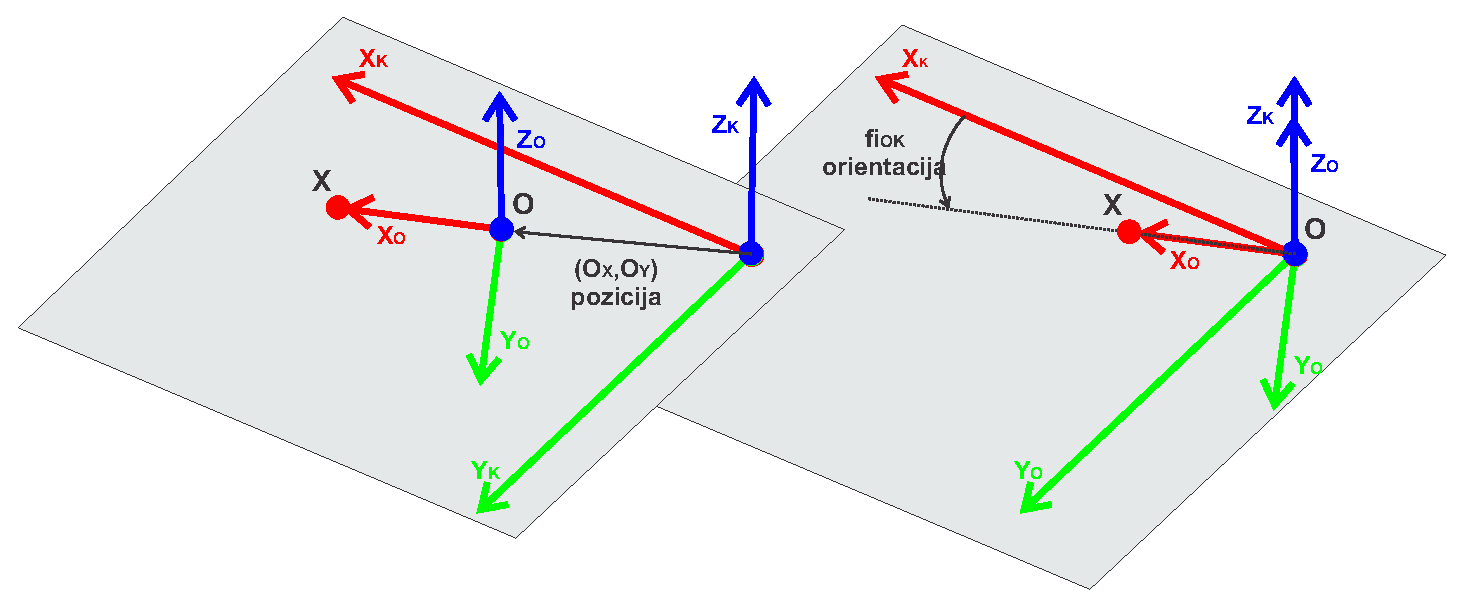
\includegraphics[width=0.85\textwidth]{/Eps/22_Lega_glede_na_kamero.eps}
    \vspace{-0.3cm}
    \caption{Lega koordinatnega sistema objekta v koordinatnem sistemu kamere}
    \label{fTransfOK}
\end{figure}

\noindent %
\textbf{\underline{Določitev matrike KamRef}} %

\vspace{0.3cm}%
Da lahko s pomočjo robotskega vida z robotom prijemamo objekte v
vidnem polju kamere in delovnem prostoru robota, je potrebno lego
objektov definirati v referenčnem koordinatnem sistemu robota. Glede
na enačbo \ref{eEqSimple} za izračun željene lege objekta v
referenčnem koordinatnem sistemu robota, potrebujemo še
\textbf{transformacijsko matriko KamRef}.
\\
\\
\noindent %
\textbf{Postopek za določitev matrike KamRef} %
\vspace{0.1cm}\\
\begin{mdframed}[backgroundcolor=green!20, shadow=true,roundcorner=8pt]
%\begin{tikzpicture}
%    \node [fill=green,rounded corners=5pt] {
%    \begin{minipage}{0.93\textwidth}
        \vspace{0.1cm}
Lega objekta oziroma koordinatnega sistema objekta je zapisana v
transformacijski matriki \textbf{ObjKam}. Za določitev lege
koordinatnega sistema kamere v referenčnem koordinatnem sistemu
robota ni mogoče najti postopka, ki bi lego določil, kot smo to
storili za lego objekta v koordinatnem sistemu kamere. Izkaže se, da
lahko postopek za določitev lege objekta v koordinatnem sistemu
kamere, v rahlo spremenjeni obliki, uporabimo za določitev matrike
\textbf{VrhRef}. Ta ob prijemu objekta predstavlja lego objekta v
referenčnem koordinatnem sistemu robota. Na ta način lahko z
izračunom določimo matriko \textbf{KamRef}, ki predstavlja lego
kamere v referenčnem koordinatnem sistemu robota.
        \vspace{0.1cm}
%    \end{minipage}
%    };
%\end{tikzpicture}
\end{mdframed}

\begin{figure}[!h]
    \center
    \includegraphics[width=0.4\textwidth]{/Eps/23_Konica.eps}
    \vspace{-0.3cm}
    \caption{V ustje robota nameščena konica, ki smo jo pozicionirali v središče točke O}
    \label{fKonica}
\end{figure}
\begin{enumerate}

\item[1)] V Epson RC+ okolju v mapi Projects\textbackslash odprite že pripravljen projekt z imenom \textbf{Epson\_kalibracija}.

\item[2)] Z ukazom \textit{Run -> Start -> Start main} projekt prevedete in zaženete.

\item[3)] Robot pobere kalibracijsko konico in se premakne do točke \emph{O}(\emph{O}$_x$, \emph{O}$_y$). Koordinate točke v World koordinatnem sistemu (Slika \ref{fUkaziPremikanjeRobota}) se izpišejo v konzoli.

\item[4)] S pritiskom na ukaz \textit{Continue} robota premaknete na točko \emph{X}(\emph{X}$_x$, \emph{X}$_y$). Koordinate točke v World koordinatnem sistemu (Slika \ref{fUkaziPremikanjeRobota}) se zopet izpišejo v konzoli.

\item[5)] S ponovnim pritiskom na ukaz \textit{Continue} robotu ukažete, da odloži kalibracijsko konico.

\item[6)] Odčitana točka \emph{O} predstavlja \textbf{pozicijo}
koordinatnega sistema objekta v referenčnem koordinatnem sistemu
robota (Slika \ref{fTransfOR}, levo). \textbf{Orientacijo}
koordinatnega sistema objekta v referenčnem koordinatnem sistemu
robota pa določa kot (fiOR) med osema \emph{X}$_R$ in \emph{X}$_O$
(Slika \ref{fTransfOR}, desno).

\begin{figure}[h]
    \center
    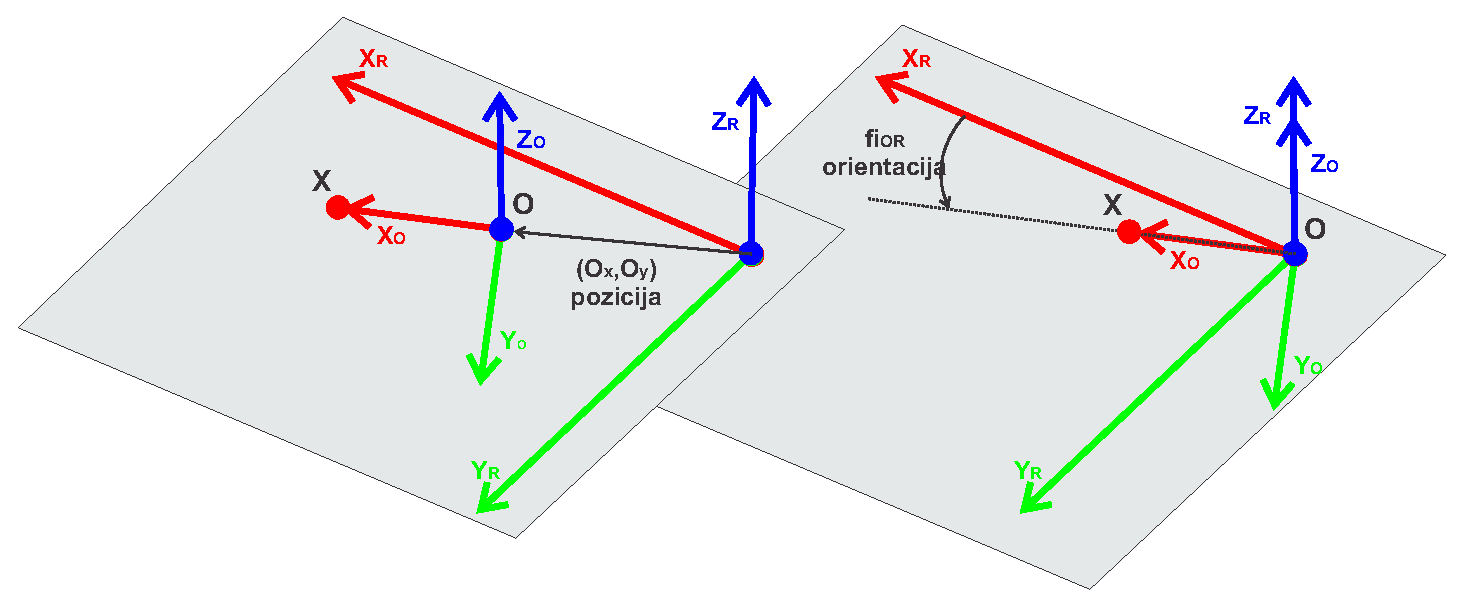
\includegraphics[width=0.85\textwidth]{/Eps/24_Lega_glede_na_bazo.eps}
    \vspace{-0.3cm}
    \caption{Lega koordinatnega sistema objekta v referenčnem koordinatnem sistemu robota}
    \label{fTransfOR}
\end{figure}

\item[7)] V okolju Matlab je že odprta datoteka
\textbf{zamaski2.m}, zato nadaljujete: \\%
\\
\small
\textcolor[rgb]{0.50,0.50,0.50}{\texttt{$\%$ V ustrezna polja vpišemo prebrane vrednosti koordinate}} \\%
\textcolor[rgb]{0.50,0.50,0.50}{\texttt{$\%$ O(O$_x$,O$_y$) in X(X$_x$,X$_y$).}} \\%
\texttt{Ox$\_$r = \emph{vpišemo prebrano koordinato};}  \\%
\texttt{Oy$\_$r = \emph{vpišemo prebrano koordinato};}  \\%
\texttt{Xx$\_$r = \emph{vpišemo prebrano koordinato};}  \\%
\texttt{Xy$\_$r = \emph{vpišemo prebrano koordinato};}  \\%
\\
\textcolor[rgb]{0.50,0.50,0.50}{\texttt{$\%$ Izračunamo kot zasuka koordinatnega sistema Objekta}} \\%
\textcolor[rgb]{0.50,0.50,0.50}{\texttt{$\%$ glede na referenčni k.s. (Slika \ref{fTransfOR}, desno).}} \\%
%\texttt{fiOR = atan2( (Xy$\_$r - Oy$\_$r ) , (Xx$\_$r - Ox$\_$r ) );} \\ %
\texttt{fiOR = \emph{... TUKAJ ZAPIŠETE PRAVILNO KODO};} \\ %
\\
\textcolor[rgb]{0.50,0.50,0.50}{\texttt{$\%$ Zapišemo transformacijsko matriko Vrh- translacija}} \\%
\textcolor[rgb]{0.50,0.50,0.50}{\texttt{$\%$ D(Ox$\_$r, Oy$\_$r) in rotacija okrog osi Z za kot fiOR.}} \\%
\texttt{VrhRef = \emph{... TUKAJ ZAPIŠETE PRAVILNO KODO};} \\ %
%\texttt{VrhRef = [cos(fiOR), -sin(fiOR), 0, Ox$\_$r; sin(fiOR), cos(fiOR),\\\hspace*{1.7cm} 0, Oy$\_$r; 0, 0, 1, 0; 0, 0, 0, 1 ];} \\ %

\normalsize %
Zapis v matrični obliki izgleda tako:
\\
\begin{equation}
    \textbf{VrhRef} =
    \begin{bmatrix}
        \textbf{cos(fiOR)}  &   \textbf{-sin(fiOR)}   &    \textbf{0}  &   \emph{Ox$\_$r}    \\%
        \textbf{sin(fiOR)}  &   \hspace{0.1cm} \textbf{cos(fiOR)}   &    \textbf{0}  &   \emph{Oy$\_$r}    \\%
        \textbf{0}              &   \textbf{0}                &    \textbf{1}  &   \emph{0}    \\%
        0              &   0                &    0  &   1     \\%
    \end{bmatrix}
    \label{eVrhRef}
\end{equation}
\\
\begin{mdframed}[backgroundcolor=blue!20, shadow=true,roundcorner=8pt]
%\begin{tikzpicture}
%    \node [fill=blue,rounded corners=5pt] {
%    \begin{minipage}{0.93\textwidth}
        \vspace{0.1cm}
Enačba \ref{eVrhRef} predstavlja transformacijsko matriko
\textbf{VrhRef} in opisuje lego objekta oziroma koordinatnega
sistema objekta v referenčnem koordinatnem sistemu robota.
        \vspace{0.1cm}
%    \end{minipage}
%    };
%\end{tikzpicture}
\end{mdframed}

\item[8)] V tem trenutku sta določeni obe transformaciji \textbf{ObjKam} in
\textbf{VrhRef}, zato lahko po spodnjem postopku izračunamo lego
koordinatnega sistema kamere v referenčnem koordinatnem sistemu
robota, ki jo predstavlja transformacijska matrika \textbf{KamRef}.
Izhodišče je enačba \ref{eEqSimple}.

\vspace{0.4cm} %

\noindent %
\begin{mdframed}[backgroundcolor=green!20, shadow=true,roundcorner=8pt]
%\begin{tikzpicture}
%    \node [fill=green,rounded corners=5pt] {
%    \begin{minipage}{0.94\textwidth}
        \vspace{0.1cm}
        \center
        \textbf{VrhRef = KamRef $\bullet$  ObjKam} \emph{$/$ z desne množimo z \textbf{(ObjKam)$^{-1}$}}\\ %
%        \textbf{EndEff = T$\_$cam2ref $\bullet$ T$\_$obj2cam $\bullet$ T$\_$grip2obj}\\ %
        \vspace{0.2cm}
        \textbf{VrhRef $\bullet$ (ObjKam)$^{-1}$ = KamRef $\bullet$ ObjKam $\bullet$ (ObjKam)$^{-1}$}\\ %
        \vspace{0.2cm}
        \textbf{KamRef = VrhRef $\bullet$ (ObjKam)$^{-1}$}\\ %
        \vspace{0.1cm}
%    \end{minipage}
%    };
%\end{tikzpicture}
\end{mdframed}
\vspace{0.0cm} %

V .m datoteko dopišete potrebne vrstice. \\ %
\\
\small
\textcolor[rgb]{0.50,0.50,0.50}{\texttt{$\%$ Zapišemo izračun transformacije KamRef}} \\%
\texttt{KamRef = \emph{... TUKAJ ZAPIŠETE PRAVILNO KODO};}  \\% ... TUKAJ ZAPIŠETE KODO;
\\
%\texttt{KamRef = VrhRef * inv(ObjKam);}  \\% ... TUKAJ ZAPIŠETE KODO;
\normalsize %

\item[9)] Ukaz \textbf{extobject2} vam bo vrnila spremenljivko \textbf{centers} v kateri se nahajajo koordinate zamaškov v enotah pixel (slikovni elementi), ki jih je potrebno pretvoriti v enote mm (milimetri). Koordinate zamaškov v enotah mm se shrani v spremeljivko \textbf{obj}.

\small
\textcolor[rgb]{0.50,0.50,0.50}{\texttt{$\%$ Središča objektov na sliki pretvorimo v metrične enote}} \\%
\texttt{obj = \emph{... TUKAJ ZAPIŠETE PRAVILNO KODO};} \\ %
\\

\normalsize %
\item[10)]  Sedaj je potrebno v izračunati matriko \textbf{VrhRef} v kateri so zapisane koordinate zamaškov v koordinatnem sistemu robota. %

~\\
\textcolor[rgb]{0.50,0.50,0.50}{\texttt{$\%$ Določitev koordinat prepoznanih objektov v referenčnem}} \\%
\textcolor[rgb]{0.50,0.50,0.50}{\texttt{$\%$ koordinatnem sistemu. Ker imamo opraviti samo s pozicijami}} \\%
\textcolor[rgb]{0.50,0.50,0.50}{\texttt{$\%$ središč pokrovčkov, ni potrebno izvajati rotacij. Zato}} \\%
\textcolor[rgb]{0.50,0.50,0.50}{\texttt{$\%$ transformacijske matrike vsebujejo samo translacijski del.}} \\%
\texttt{for ii = 1:size(centers,1)} \\ %
%\hspace*{0.2 cm}\texttt{ObjKam = [1,0,0,obj(ii,1); 0,1,0,obj(ii,2); 0,0,1,Z; 0,0,0,1];} \\ %
%\hspace*{0.2 cm}\texttt{VrhRef(:,:,ii) = KamRef * ObjKam;} \\ %
\hspace*{0.2 cm}\texttt{ObjKam = \emph{... TUKAJ ZAPIŠETE PRAVILNO KODO};} \\ %
\hspace*{0.2 cm}\texttt{VrhRef(:,:,ii) = \emph{... TUKAJ ZAPIŠETE PRAVILNO KODO};} \\ %
\texttt{end} \\ %
\\
\textcolor[rgb]{0.50,0.50,0.50}{\texttt{$\%$ Iz serije transformacijskih matrik Vrh izluščimo samo}} \\%
\textcolor[rgb]{0.50,0.50,0.50}{\texttt{$\%$ koordinate središč zamaškov v referenčnem k.s.}} \\%
\texttt{koord$\_$zamaskov;} \\ %

\normalsize %
\item[11)]  \textbf{Datoteko zamaski2.m shranimo in preverimo kalibracijo:} %

\end{enumerate}
\normalsize

\begin{mdframed}[backgroundcolor=red!20, shadow=true,roundcorner=8pt]
\begin{itemize}
  \item \textbf{Asistent naj iz mizice odstrani kalibracijsko ploščo in na mizico postavi tri zamaške.}
  \item \textbf{Zamaški naj se nahajajo v kotih, kjer so na kalibracijski mizici kalibracijske točke.}
\end{itemize}
\end{mdframed}

Kalibracijo preverite tako, da z ukazom \\

\vspace{-0.3cm}%
\textbf{$\gg$ extobject2} \verb"Enter"\\ %\Enter
\vspace{-0.1cm}%

odprete okno za zajem slike zamaškov. S ponovnim pritiskom tipke \verb"Enter" sliko zajamete. Z ukazom  \\

\vspace{-0.3cm}%
\textbf{$\gg$ zamaski2} \verb"Enter" \\%\Enter
\vspace{-0.1cm}%

se izračunajo in izpišejo koordinate zamaškov v globalnem koordinatnem sistemu. Izpisane koordinate primerjate s pozicijami kalibracijskih točk, ki ste jih dobili v prejšnjem postopku. Koordinate se morajo približno ujemati (\texttildelow$\pm1mm$).

\vspace{-0.2cm}
\subsection{Koraki za zagon}
\vspace{0.3cm} %

\begin{mdframed}[backgroundcolor=red!20, shadow=true,roundcorner=8pt]
\begin{itemize}
  \item \textbf{Asistent naj na mizico postavi več zamaškov.}
  \item \textbf{Med izvajanjem mora biti asistent ves čas pri robotu}
\end{itemize}
\end{mdframed}

\begin{enumerate}


\item[1)] \textbf{Vsi postopki določanja
transformacijskih matrik ObjKam in KamRef ter vse vrstice programska
kode v datoteki zamaski2.m morajo biti opravljeni oziroma zapisani!} \\%

\item[2)] \textbf{V vidno polje kamere postavite nekaj zamaškov}
(recimo 7), še prej pa odstranite kalibracijsko konico, umaknete
robot iz vidnega področja kamere in odstranite list s
koordinatnim sistemom objekta. \\ %

\item[3)] V Matlab ukazni vrstici zaženete: \\ %
%\vspace{-0.1cm} %
\textbf{$\gg$ extobject2} \verb"Enter" \\ %%\Enter


Odpre se okno kamere z živo sliko za boljše pozicioniranje zamaškov.
Ko ste s pozicijo zamaškov zadovoljni, pritisnete \verb"Enter". čez čas se%%\Enter
v ukazni vrstici okolja Matlab izpiše število razpoznanih objektov
in izriše se slika \ref{fRazbraniZamaski}. \textbf{če niste
zadovoljni z razpoznavo objektov, ta korak ponovite.} %

\begin{figure}[!h]
    \center
    \includegraphics[width=0.7\textwidth]{/Eps/25_Razbrani_zamaski.eps}
    \vspace{-0.3cm}
    \caption{Iz zajete slike razbrani zamaški ter označena njihova središča}
    \label{fRazbraniZamaski}
\end{figure}

\item[4)] V ukazni vrstici okolja Matlab poženete datoteko(\emph{zamaski2.m}).  \\ %

%\vspace{-0.3cm} %
\textbf{$\gg$ zamaski2} \verb"Enter" \\ %%\Enter
\vspace{-0.1cm} %

\item[5)] V Epson RC+ okolju v mapi Projects$\backslash$ odprete že pripravljen projekt z imenom \textbf{Epson$\_$kamera}. \\ %

\begin{mdframed}[backgroundcolor=red!80, shadow=true,roundcorner=8pt]
%\begin{tikzpicture}
%    \node [fill=red,rounded corners=5pt] {
%    \begin{minipage}{0.93\textwidth}
        \vspace{0.1cm}
 \textbf{Ob zagonu programa poskrbite, da robot deluje %
 z nižjo močjo in njegova hitrost gibanja naj bo le 10$\%$ (prvi dve vrstici programa).}
 \\
 \\
\hspace*{3.5cm}\textcolor[rgb]{1.00,1.00,0.00}{\emph{\textbf{$\#$define dPower Low}}} \\ %
\hspace*{3.5cm}\textcolor[rgb]{1.00,1.00,0.00}{\emph{\textbf{$\#$define dSpeedAccelProcent 10}}} \\ %
        \vspace{-0.3cm}
%    \end{minipage}
%    };
%\end{tikzpicture}
\end{mdframed}
\vspace{0.3cm}

\item[6)] S tipko F5 projekt prevedete
(Slika \ref{fZaganjanjePrograma}) in ga zaženete s klikom na gumb \textbf{Start tcpipcomm}. %

% ********************************************************************
\vspace{0.3cm}
\begin{mdframed}[backgroundcolor=red!80, shadow=true,roundcorner=8pt]
%\begin{tikzpicture}
%    \node [fill=red,rounded corners=5pt] {
%    \begin{minipage}{0.93\textwidth}
        \vspace{0.1cm}
        \center
        \large
\textcolor[rgb]{1.00,1.00,0.00}{\LARGE\textbf{OPOZORILO!}}\\ %
\textcolor[rgb]{1.00,1.00,0.00}{\large Pred zagonom programa je
potrebno zagotoviti, da v delovnem prostoru ni osebe ali predmeta, s
katerim bi lahko robot trčil.} \\ %
        \vspace{0.1cm}
%    \end{minipage}
%    };
%\end{tikzpicture}
\end{mdframed}
\vspace{0.3cm}
\item[7)] V ukazni vrstici okolja Matlab izvršite ukaz (štarta premikanje robota): \\ %

\vspace{-0.1cm} %
\textbf{$\gg$ zamaski$\_$tcp} \verb"Enter" \\ %%\Enter
\normalsize
% ********************************************************************
\end{enumerate}
